\documentclass[11pt,]{article}
\usepackage[]{mathpazo}
\usepackage{amssymb,amsmath}
\usepackage{ifxetex,ifluatex}
\usepackage{fixltx2e} % provides \textsubscript
\ifnum 0\ifxetex 1\fi\ifluatex 1\fi=0 % if pdftex
  \usepackage[T1]{fontenc}
  \usepackage[utf8]{inputenc}
\else % if luatex or xelatex
  \ifxetex
    \usepackage{mathspec}
  \else
    \usepackage{fontspec}
  \fi
  \defaultfontfeatures{Ligatures=TeX,Scale=MatchLowercase}
\fi
% use upquote if available, for straight quotes in verbatim environments
\IfFileExists{upquote.sty}{\usepackage{upquote}}{}
% use microtype if available
\IfFileExists{microtype.sty}{%
\usepackage{microtype}
\UseMicrotypeSet[protrusion]{basicmath} % disable protrusion for tt fonts
}{}
\usepackage[margin=1in]{geometry}
\usepackage{hyperref}
\hypersetup{unicode=true,
            pdftitle={Case Study: Predicting the outcomes of the 2017 Dutch General Elections},
            pdfauthor={Ilse van Beelen, Floor Komen},
            pdfkeywords={put some keywords here},
            pdfborder={0 0 0},
            breaklinks=true}
\urlstyle{same}  % don't use monospace font for urls
\usepackage{natbib}
\bibliographystyle{plainnat}
\usepackage{color}
\usepackage{fancyvrb}
\newcommand{\VerbBar}{|}
\newcommand{\VERB}{\Verb[commandchars=\\\{\}]}
\DefineVerbatimEnvironment{Highlighting}{Verbatim}{commandchars=\\\{\}}
% Add ',fontsize=\small' for more characters per line
\usepackage{framed}
\definecolor{shadecolor}{RGB}{248,248,248}
\newenvironment{Shaded}{\begin{snugshade}}{\end{snugshade}}
\newcommand{\KeywordTok}[1]{\textcolor[rgb]{0.13,0.29,0.53}{\textbf{#1}}}
\newcommand{\DataTypeTok}[1]{\textcolor[rgb]{0.13,0.29,0.53}{#1}}
\newcommand{\DecValTok}[1]{\textcolor[rgb]{0.00,0.00,0.81}{#1}}
\newcommand{\BaseNTok}[1]{\textcolor[rgb]{0.00,0.00,0.81}{#1}}
\newcommand{\FloatTok}[1]{\textcolor[rgb]{0.00,0.00,0.81}{#1}}
\newcommand{\ConstantTok}[1]{\textcolor[rgb]{0.00,0.00,0.00}{#1}}
\newcommand{\CharTok}[1]{\textcolor[rgb]{0.31,0.60,0.02}{#1}}
\newcommand{\SpecialCharTok}[1]{\textcolor[rgb]{0.00,0.00,0.00}{#1}}
\newcommand{\StringTok}[1]{\textcolor[rgb]{0.31,0.60,0.02}{#1}}
\newcommand{\VerbatimStringTok}[1]{\textcolor[rgb]{0.31,0.60,0.02}{#1}}
\newcommand{\SpecialStringTok}[1]{\textcolor[rgb]{0.31,0.60,0.02}{#1}}
\newcommand{\ImportTok}[1]{#1}
\newcommand{\CommentTok}[1]{\textcolor[rgb]{0.56,0.35,0.01}{\textit{#1}}}
\newcommand{\DocumentationTok}[1]{\textcolor[rgb]{0.56,0.35,0.01}{\textbf{\textit{#1}}}}
\newcommand{\AnnotationTok}[1]{\textcolor[rgb]{0.56,0.35,0.01}{\textbf{\textit{#1}}}}
\newcommand{\CommentVarTok}[1]{\textcolor[rgb]{0.56,0.35,0.01}{\textbf{\textit{#1}}}}
\newcommand{\OtherTok}[1]{\textcolor[rgb]{0.56,0.35,0.01}{#1}}
\newcommand{\FunctionTok}[1]{\textcolor[rgb]{0.00,0.00,0.00}{#1}}
\newcommand{\VariableTok}[1]{\textcolor[rgb]{0.00,0.00,0.00}{#1}}
\newcommand{\ControlFlowTok}[1]{\textcolor[rgb]{0.13,0.29,0.53}{\textbf{#1}}}
\newcommand{\OperatorTok}[1]{\textcolor[rgb]{0.81,0.36,0.00}{\textbf{#1}}}
\newcommand{\BuiltInTok}[1]{#1}
\newcommand{\ExtensionTok}[1]{#1}
\newcommand{\PreprocessorTok}[1]{\textcolor[rgb]{0.56,0.35,0.01}{\textit{#1}}}
\newcommand{\AttributeTok}[1]{\textcolor[rgb]{0.77,0.63,0.00}{#1}}
\newcommand{\RegionMarkerTok}[1]{#1}
\newcommand{\InformationTok}[1]{\textcolor[rgb]{0.56,0.35,0.01}{\textbf{\textit{#1}}}}
\newcommand{\WarningTok}[1]{\textcolor[rgb]{0.56,0.35,0.01}{\textbf{\textit{#1}}}}
\newcommand{\AlertTok}[1]{\textcolor[rgb]{0.94,0.16,0.16}{#1}}
\newcommand{\ErrorTok}[1]{\textcolor[rgb]{0.64,0.00,0.00}{\textbf{#1}}}
\newcommand{\NormalTok}[1]{#1}
\usepackage{graphicx,grffile}
\makeatletter
\def\maxwidth{\ifdim\Gin@nat@width>\linewidth\linewidth\else\Gin@nat@width\fi}
\def\maxheight{\ifdim\Gin@nat@height>\textheight\textheight\else\Gin@nat@height\fi}
\makeatother
% Scale images if necessary, so that they will not overflow the page
% margins by default, and it is still possible to overwrite the defaults
% using explicit options in \includegraphics[width, height, ...]{}
\setkeys{Gin}{width=\maxwidth,height=\maxheight,keepaspectratio}
\IfFileExists{parskip.sty}{%
\usepackage{parskip}
}{% else
\setlength{\parindent}{0pt}
\setlength{\parskip}{6pt plus 2pt minus 1pt}
}
\setlength{\emergencystretch}{3em}  % prevent overfull lines
\providecommand{\tightlist}{%
  \setlength{\itemsep}{0pt}\setlength{\parskip}{0pt}}
\setcounter{secnumdepth}{0}
% Redefines (sub)paragraphs to behave more like sections
\ifx\paragraph\undefined\else
\let\oldparagraph\paragraph
\renewcommand{\paragraph}[1]{\oldparagraph{#1}\mbox{}}
\fi
\ifx\subparagraph\undefined\else
\let\oldsubparagraph\subparagraph
\renewcommand{\subparagraph}[1]{\oldsubparagraph{#1}\mbox{}}
\fi

%%% Use protect on footnotes to avoid problems with footnotes in titles
\let\rmarkdownfootnote\footnote%
\def\footnote{\protect\rmarkdownfootnote}

%%% Change title format to be more compact
\usepackage{titling}

% Create subtitle command for use in maketitle
\newcommand{\subtitle}[1]{
  \posttitle{
    \begin{center}\large#1\end{center}
    }
}

\setlength{\droptitle}{-2em}

  \title{Case Study: Predicting the outcomes of the 2017 Dutch General Elections}
    \pretitle{\vspace{\droptitle}\centering\huge}
  \posttitle{\par}
    \author{Ilse van Beelen, Floor Komen}
    \preauthor{\centering\large\emph}
  \postauthor{\par}
      \predate{\centering\large\emph}
  \postdate{\par}
    \date{January 18, 2019}

\usepackage{float}

\begin{document}
\maketitle
\begin{abstract}
Put the abstract over here
\end{abstract}

\section{1. Introduction}\label{introduction}

\subsection{1.1 Motivation}\label{motivation}

For this case study, it was decided to combine the outcome from the
Dutch elections of 2017 and demographic data. Both are collected per
municipality and are well maintained and reliable. This makes A lot of
information is available for both in the Netherlands. This will
hopefully result in observing voting trends per demographic group. The
final goal is to validate the model for making futyre predictions.

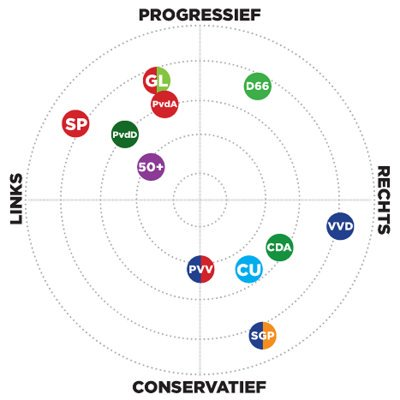
\includegraphics[width=2.60417in]{Partijlandschap.jpg} \textbf{Dutch
political parties}\\
This figure displays the diffences between the political parties in the
Netherlands. The Netherlands has a total of 13 parties. This
investigation focusses on only one party. This party should not be to
extreme left/right/conservative/progressive and should also be one of
the bigger parties. Otherwise, there is not enough data available,
making the results less reliable. Therefore, party CDA is chosen.

In this research the above described demographics are chosen because of
their influence on a municipality level. The expectation is that a
municipality with more non-western residents for example votes different
than a municipality with less non-western residents. This is the same
for the other two demographics. Other demographics are also researched,
for example gender, but on a municipality level there is no large
difference between the amount of men and women per municipality. So that
is a more interesting demographic to research on an individual level.
\emph{The standardized income per municipality} are given in thousands.
\emph{the urban index of a municipality} is a database with five
categories per municipality. These five categories are:

\begin{itemize}
\item Really strong urbanity (more than 2500 addresses per $km^2$) 
\item Strong urbanity (1500-2500 addresses per $km^2$) 
\item Moderate urbanity (1000- 1500 addresses per $km^2$) 
\item Little urbanity (500-1000 addresses per $km^2$)  
\item No urbanity (less than 500 addresses per $km^2$)
\end{itemize}

Per municipality the amount of \(km^2\) per category is given. The
\emph{non-west residents per municipality} is given in an amount per
municipality, also the total amount of residents is given per
municipality.

\subsection{1.2 Data sources}\label{data-sources}

\textbf{Electoral data} For the electoral data, the results of the 2017
general election are used. This is the most recent national election and
is of the most important election type in the Netherlands. Furthermore,
it had a turnup of 81.9\%. Therefore, it seems plausible that the data
for this election is representative of the political makeup of different
municipalities. We downloaded the raw data directly from the official
government source.\footnote{\url{https://data.overheid.nl/data/dataset/verkiezingsuitslag-tweede-kamer-2017}}
This contained a .csv file with the raw number of votes for every party
in every municipality.

\textbf{Demographical data}\\
We got our demographical data from the CBS, the official Dutch
statistical agency.\footnote{\url{https://opendata.cbs.nl/statline/\#/CBS/nl/dataset/70072ned/table?ts=1544803364892}}
From the wealth of demographical information available we picked a
handful of attributes that we suspected (based on prior research and
some gut feeling) to be useful as predictor variables. We landed on five
demographical attributes: education grade, average income, age,
urbanization and the amount of people with a non-western background.
Note that the data we downloaded from the CBS site usually had to be
transformed to get it in a useful predictor variable format. The
specifics of these are described in the next section.

\subsection{1.3 Data cleaning}\label{data-cleaning}

An extensive amount of data cleaning had to be done. Below these steps
are describes and a small part of code is displayed.

\textbf{Electoral data}

\textbf{Demographical data}

The variable \emph{non-western residents} are divided in three groups:

\begin{itemize}
\item Municipalities with less than 5 % non-western residents 
\item Municipalities with 5-10 % non-western resident 
\item Municipalities with mre than 10 % non-western residents
\end{itemize}

\begin{Shaded}
\begin{Highlighting}[]
\NormalTok{Data_CDA}\OperatorTok{$}\NormalTok{Non_west <-}\StringTok{ }\KeywordTok{ifelse}\NormalTok{(Data_CDA}\OperatorTok{$}\NormalTok{Non_west_frac }\OperatorTok{<}\StringTok{ }\FloatTok{0.05}\NormalTok{, }\DecValTok{1}\NormalTok{, }\OtherTok{NA}\NormalTok{)}
\NormalTok{Data_CDA}\OperatorTok{$}\NormalTok{Non_west <-}\StringTok{ }\KeywordTok{ifelse}\NormalTok{(Data_CDA}\OperatorTok{$}\NormalTok{Non_west_frac }\OperatorTok{>=}\StringTok{ }\FloatTok{0.05} \OperatorTok{&}\StringTok{ }\NormalTok{Data_CDA}\OperatorTok{$}\NormalTok{Non_west_frac }\OperatorTok{<}\StringTok{ }
\StringTok{    }\FloatTok{0.1}\NormalTok{, }\DecValTok{2}\NormalTok{, Data_CDA}\OperatorTok{$}\NormalTok{Non_west)}
\NormalTok{Data_CDA}\OperatorTok{$}\NormalTok{Non_west <-}\StringTok{ }\KeywordTok{ifelse}\NormalTok{(Data_CDA}\OperatorTok{$}\NormalTok{Non_west_frac }\OperatorTok{>=}\StringTok{ }\FloatTok{0.1}\NormalTok{, }\DecValTok{3}\NormalTok{, Data_CDA}\OperatorTok{$}\NormalTok{Non_west)}
\NormalTok{Data_CDA}\OperatorTok{$}\NormalTok{Non_west <-}\StringTok{ }\KeywordTok{as.factor}\NormalTok{(Data_CDA}\OperatorTok{$}\NormalTok{Non_west)}
\end{Highlighting}
\end{Shaded}

At last, the electoral data and demographic data are combined again.
Only the municipality Boxmeer is removed, due to a mistake not all the
votes are reported here\footnote{\url{https://www.gelderlander.nl/boxmeer/7-600-stemmen-in-boxmeer-niet-meegenomen-in-uitslag-verkiezingen~a063ee9e/}}.
The final dataset has no NAs

\begin{Shaded}
\begin{Highlighting}[]
\KeywordTok{summary}\NormalTok{(Data_CDA)}
\end{Highlighting}
\end{Shaded}

\begin{verbatim}
##      Muni              CDA_frac       Urban_index     High_educated_frac
##  Length:366         Min.   :0.0310   Min.   :0.0000   Min.   :0.1200    
##  Class :character   1st Qu.:0.1170   1st Qu.:0.6623   1st Qu.:0.2200    
##  Mode  :character   Median :0.1420   Median :1.2305   Median :0.2600    
##                     Mean   :0.1528   Mean   :1.4280   Mean   :0.2662    
##                     3rd Qu.:0.1820   3rd Qu.:2.1750   3rd Qu.:0.3000    
##                     Max.   :0.4200   Max.   :3.7890   Max.   :0.4700    
##   Mean_income    Non_west_frac        CDA_abs        Total_abs     
##  Min.   :20.80   Min.   :0.01000   Min.   :  421   Min.   :  2727  
##  1st Qu.:24.30   1st Qu.:0.03000   1st Qu.: 1737   1st Qu.: 11516  
##  Median :25.60   Median :0.05000   Median : 2510   Median : 16915  
##  Mean   :25.91   Mean   :0.06574   Mean   : 3254   Mean   : 25162  
##  3rd Qu.:27.00   3rd Qu.:0.08000   3rd Qu.: 4023   3rd Qu.: 27087  
##  Max.   :41.80   Max.   :0.38000   Max.   :18813   Max.   :440854  
##   Frac_60plus     Non_west
##  Min.   :0.0700   1:178   
##  1st Qu.:0.1200   2:111   
##  Median :0.1300   3: 77   
##  Mean   :0.1327           
##  3rd Qu.:0.1400           
##  Max.   :0.1800
\end{verbatim}

\subsection{1.3 Data visualisation}\label{data-visualisation}

In this part the cleaned data is visualized, so that a good picture can
be obtained of the current data. First of all some demographics of data
will be showed. In figure \ref{1} of the \emph{parties}, \emph{the urban
index}, \emph{the percentage of highly educated residents}, \emph{the
mean income}, \emph{The non west residents factor} and * the percentage
60 plus* are plotted. As you can see in the plot, they are normal
distributed. Because of the low values at the x-axis, the CDA,
GroenLinks, 60 plus percentage and the highly educated densities are
above 1. The area beneath the curve sums to 1, so it is correct.

\begin{figure}[H]

{\centering 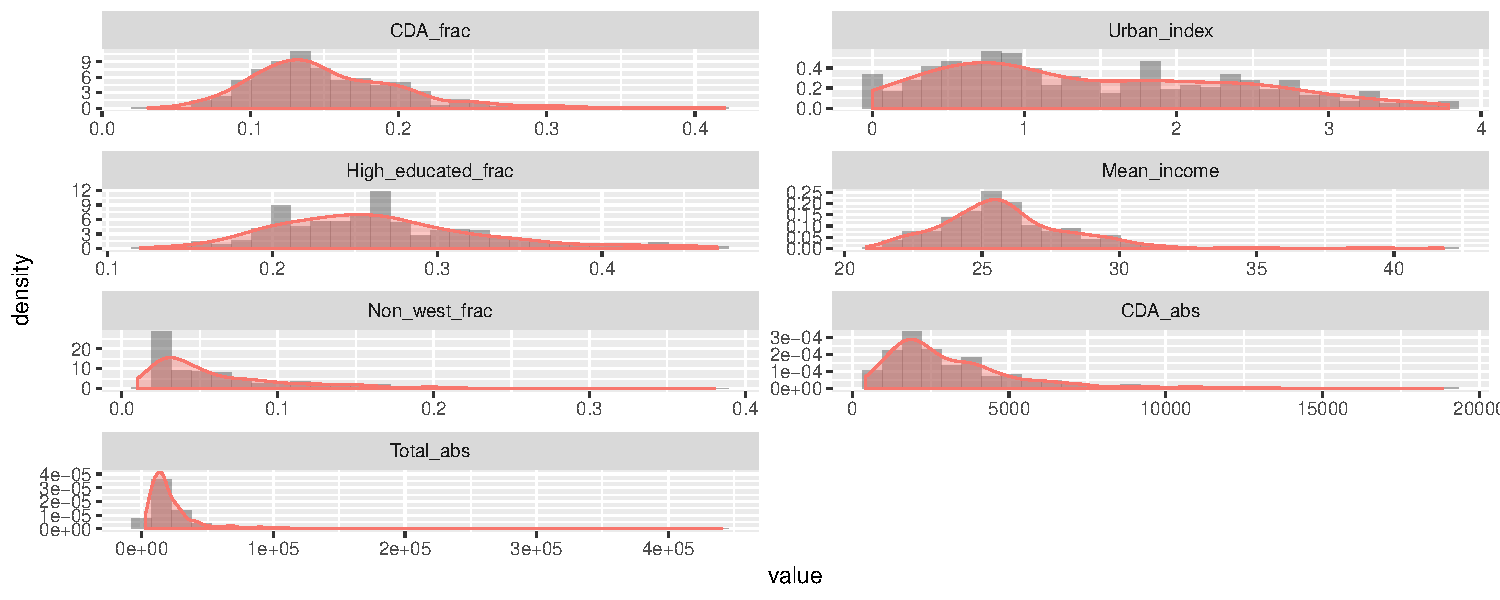
\includegraphics{Report_files/figure-latex/demographics_data-1} 

}

\caption{\label{1} Density plot}\label{fig:demographics_data}
\end{figure}

\textbf{Correlation heatmap} In this heatmap (figure \ref{2}) the
correlation between explanatory and respons variable are showed. The red
color means a positive relation, the purple color means a negative
relation. The non\_west variable is not taken into account, because it
is a factor and the other variables are continous.

\begin{figure}[H]

{\centering 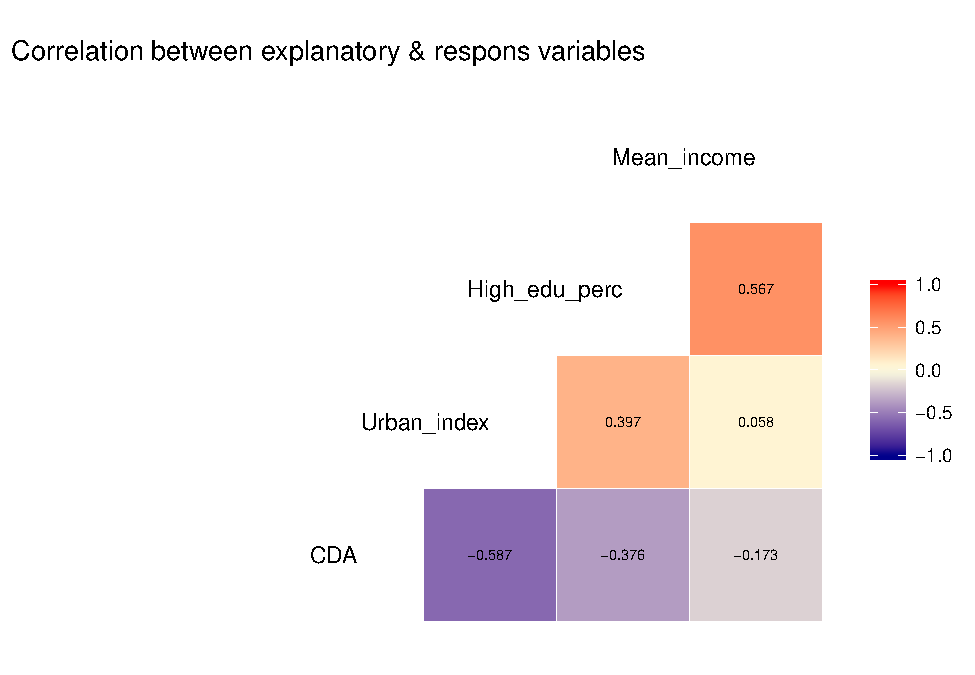
\includegraphics{Report_files/figure-latex/correlation_heatmap-1} 

}

\caption{\label{2}Correlation between explanatory and respons variables}\label{fig:correlation_heatmap}
\end{figure}

\textbf{Multilineair plots CDA } In these two plots you can see a
scatterplot with on the y-axis the votes for CDA in percentages and on
the x-axis on the left graph the mean income per municipality in 1000
euro. The right plot has the urbanity index as x-axis. As you can see,
the trend is that when the mean income goes up, the votes for CDA goes
down. Same with the urbanity index. In the model formulation graph these
trends are checked.

\begin{figure}[H]

{\centering 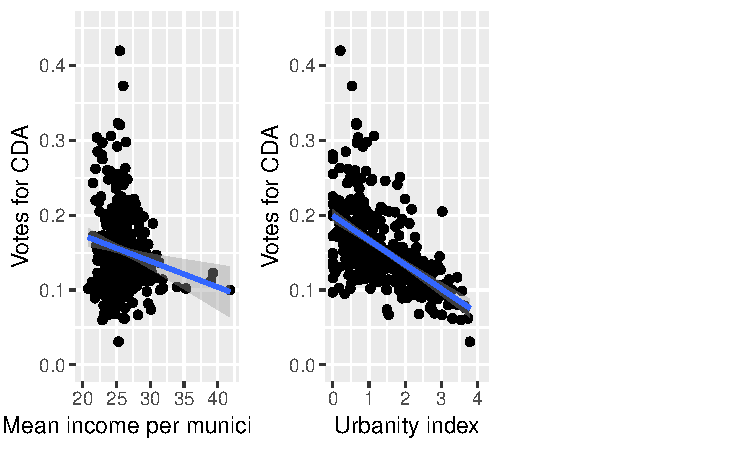
\includegraphics{Report_files/figure-latex/unnamed-chunk-6-1} 

}

\caption{\label{3}Scatterplots CDA}\label{fig:unnamed-chunk-6}
\end{figure}

\textbf{Exploratory plots of variables} These three plots are
scatterplots of the explanatory variables.

\begin{figure}[H]

{\centering 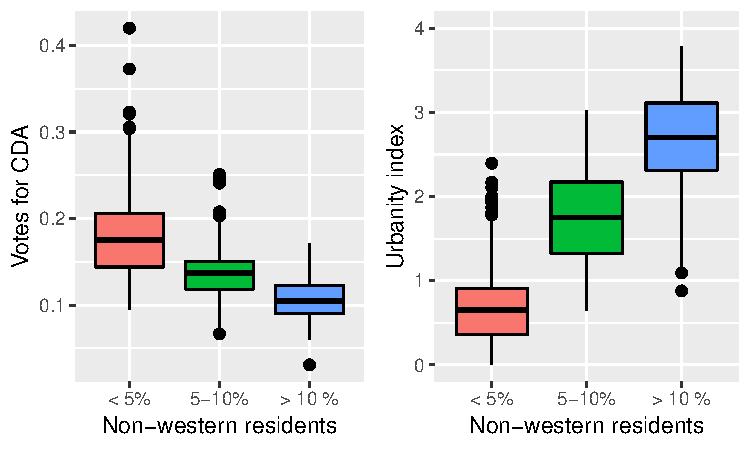
\includegraphics{Report_files/figure-latex/unnamed-chunk-7-1} 

}

\caption{\label{5}Scatterplot explanatory variables}\label{fig:unnamed-chunk-71}
\end{figure}\begin{figure}[H]

{\centering 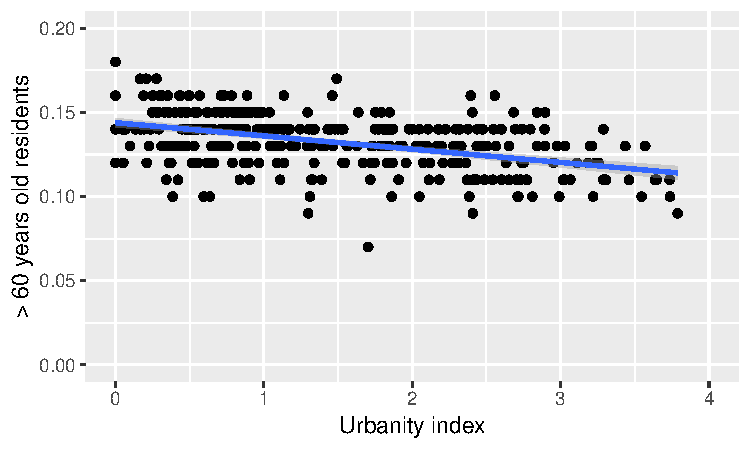
\includegraphics{Report_files/figure-latex/unnamed-chunk-7-2} 

}

\caption{\label{5}Scatterplot explanatory variables}\label{fig:unnamed-chunk-72}
\end{figure}

\textbf{Multiple boxplots} In this graph boxplots are made, to compare
some variables. A boxplot is a standardized way to display the
distribution of data. It gives the minimum, first quartile, median,
third quartile and the maximum. If there are any outliers, the boxplot
is extended with those. The line within the box is the median, the first
and third quartile are the down- and upside of the box, respectively.
The length of the box is the Inter Quartile Range (IQR). The minimum and
maximum are 1.5X Inter Quartile Range (IQR). Observations further away
can be considered outliers.

\begin{figure}[H]

{\centering 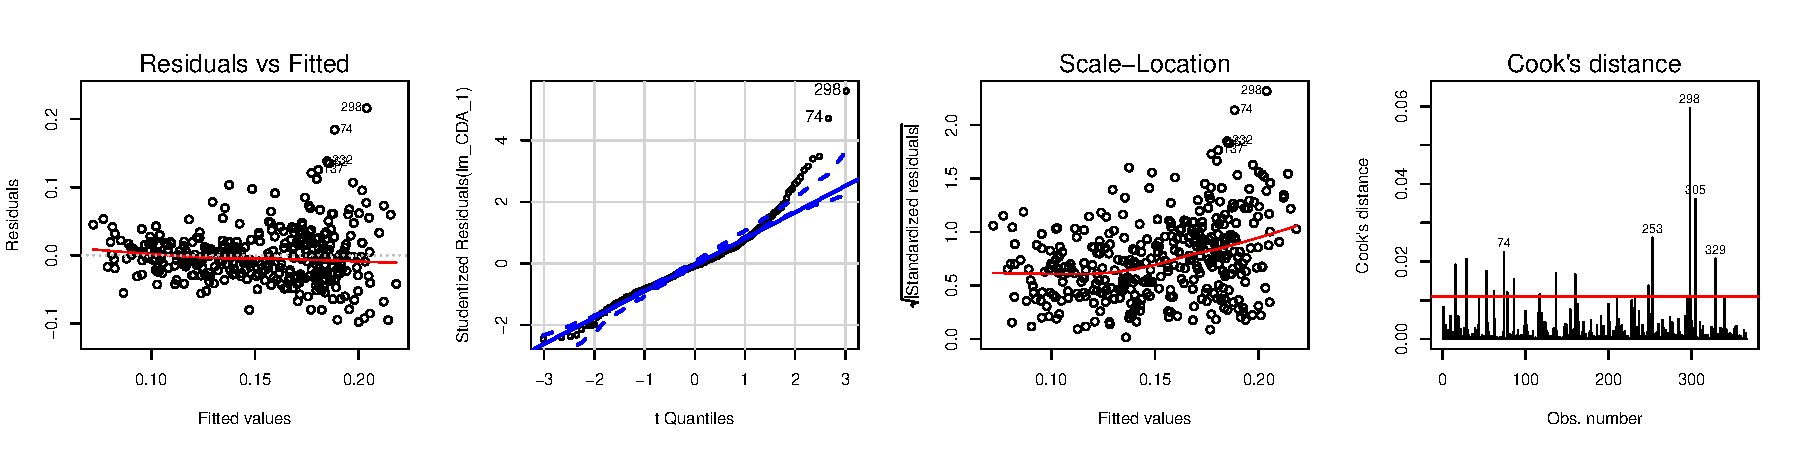
\includegraphics{Report_files/figure-latex/unnamed-chunk-8-1} 

}

\caption{\label{6}Three boxplots: Votes for CDA, Votes for GroenLinks and Urbanity index}\label{fig:unnamed-chunk-8}
\end{figure}

\section{2. Multiple linear
regression}\label{multiple-linear-regression}

In this chapter multiple linear models are generated. The demographics
tested in this model are the highly educated fraction in a municipality
\texttt{High\_educated\_frac}, the urban index of a municipality
\texttt{Urban\_index}, the mean income of the municipality
\texttt{Mean\_income}, the non-west factor \texttt{Non\_west} and the
fraction that is 60 plus in the municipality \texttt{Frac\_60plus}. The
error assumptions are also discussed. This are assumptions made for the
residuals, to check if meet the requirements for correct linear
regressions. These assumptions are: * Linearity: The expected value of
the error is zero * Constant variance: The variance of the error is
constant * Normality: The errors are normally distributed * Indepence:
The observations are sampled indipendently

\subsection{First model}\label{first-model}

The first model will be the model with all the demographics:\\
\(Y_i = \beta_0 + \beta_1*high educated fraction + \beta_2*Urban index + \beta_3*Mean income + \beta_4*Non west2 +\beta_5*Non west3 + \beta_6*Frac 60plus + \epsilon i\)\\
The outcome of this model is shown below:

\begin{table}[ht]
\centering
\begin{tabular}{rrrrr}
  \hline
 & Estimate & Std. Error & t value & Pr() \\ 
  \hline
(Intercept) & 0.3381 & 0.0314 & 10.78 & 0.0000 \\ 
  High\_educated\_frac & -0.0864 & 0.0454 & -1.90 & 0.0576 \\ 
  Urban\_index & -0.0193 & 0.0041 & -4.69 & 0.0000 \\ 
  Mean\_income & -0.0015 & 0.0011 & -1.46 & 0.1453 \\ 
  Non\_west2 & -0.0223 & 0.0065 & -3.45 & 0.0006 \\ 
  Non\_west3 & -0.0455 & 0.0095 & -4.77 & 0.0000 \\ 
  Frac\_60plus & -0.5904 & 0.1494 & -3.95 & 0.0001 \\ 
   \hline
\end{tabular}
\end{table}

The first model is the total model, \texttt{high\_educated\_frac} and
\texttt{Mean\_income} do not have a significant t-value. Before any
conclusions are made, the assumptions are checked via plots and the VIF
is checked. The VIF is the Variation Inflation Factor, it implies if
there is multicollinearity between two or more variables. The formula
for VIF is \(1/(1-R^2)\) and the thresholdvalue is 10. So values above
10 give signs of multicollinearity. As shown below none of the values
are above 10, so no signs of collinearity.

\begin{verbatim}
## High_educated_frac        Urban_index        Mean_income 
##           1.871032           3.383149           1.658015 
##          Non_west2          Non_west3        Frac_60plus 
##           1.974537           3.361734           1.289979
\end{verbatim}

\begin{verbatim}
## [1]  74 298
\end{verbatim}

\begin{figure}[H]

{\centering 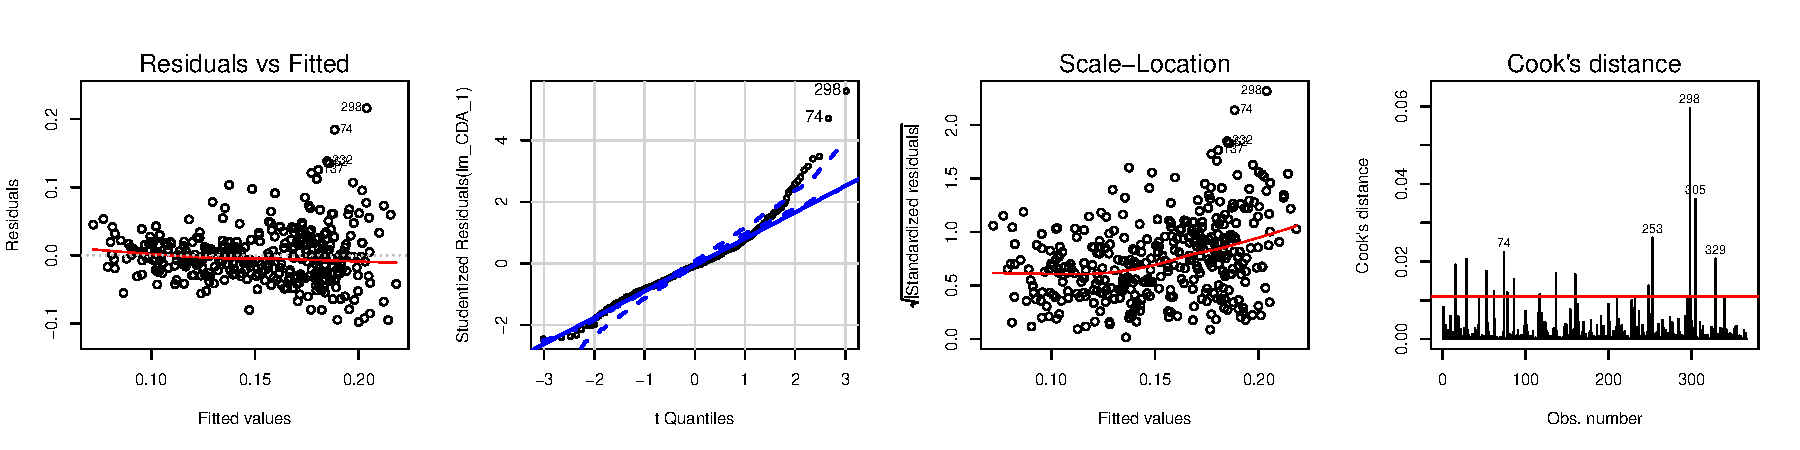
\includegraphics{Report_files/figure-latex/unnamed-chunk-9-1} 

}

\caption{\label{afm}assumptions first model}\label{fig:unnamed-chunk-9}
\end{figure}

In figure \ref{afm} the four plots are shown. The first plot (Residuals
vs Fitted) shows that the residuals have a `loudspeaker pattern', the
variance of the residuals tends to increase with an increase of the
fitted value. Because of this, a BoxCox graph is consulted. This graph
suggests a transformation for the response. The BoxCos figure \ref{BC1}
in has a 95\% Confidence interval located around the 0. So a ln
transformation is suggested.

\begin{figure}[H]

{\centering 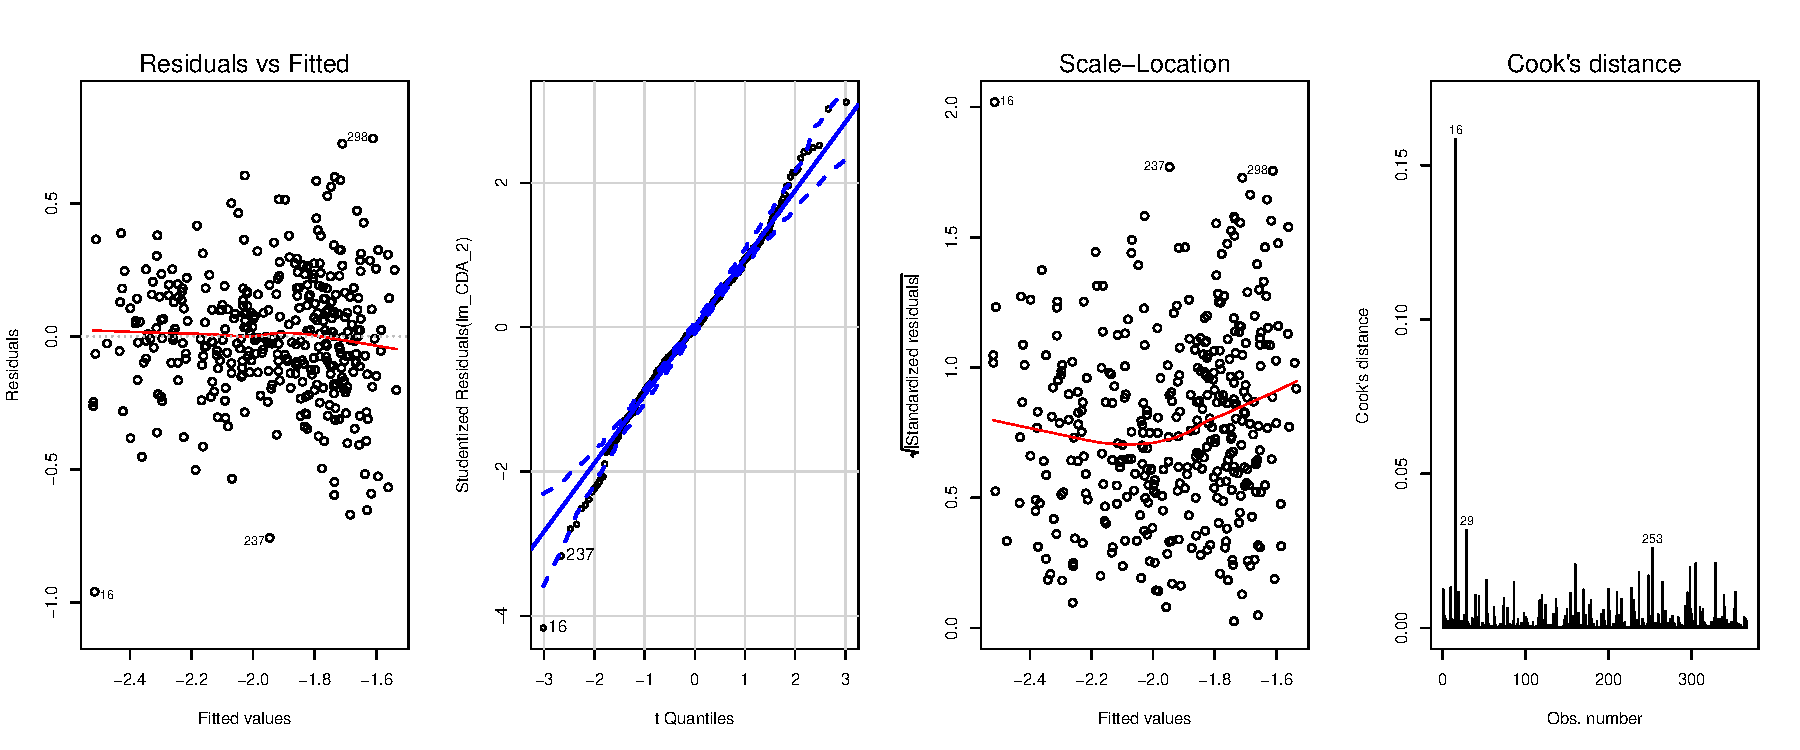
\includegraphics{Report_files/figure-latex/unnamed-chunk-10-1} 

}

\caption{\label{BC1}BoxCox first model}\label{fig:unnamed-chunk-10}
\end{figure}

\subsection{Second model}\label{second-model}

In the second model the response variable will be ln transformed. So the
new model will be:\\
\(ln(Y_i) = \beta_0 + \beta_1*high educated fraction + \beta_2*Urban index + \beta_3*Mean income + \beta_4*Non west2 + \beta_5*Non west 3 + \beta_6*Frac 60plus + \epsilon i\)

\begin{table}[ht]
\centering
\begin{tabular}{rrrrr}
  \hline
 & Estimate & Std. Error & t value & Pr() \\ 
  \hline
(Intercept) & -0.9944 & 0.1882 & -5.28 & 0.0000 \\ 
  High\_educated\_frac & -0.8808 & 0.2723 & -3.24 & 0.0013 \\ 
  Urban\_index & -0.1388 & 0.0247 & -5.62 & 0.0000 \\ 
  Mean\_income & -0.0024 & 0.0064 & -0.38 & 0.7042 \\ 
  Non\_west2 & -0.0991 & 0.0389 & -2.55 & 0.0112 \\ 
  Non\_west3 & -0.2763 & 0.0572 & -4.83 & 0.0000 \\ 
  Frac\_60plus & -2.6940 & 0.8965 & -3.01 & 0.0028 \\ 
   \hline
\end{tabular}
\end{table}

\begin{verbatim}
## [1]  16 237
\end{verbatim}

\begin{figure}[H]

{\centering 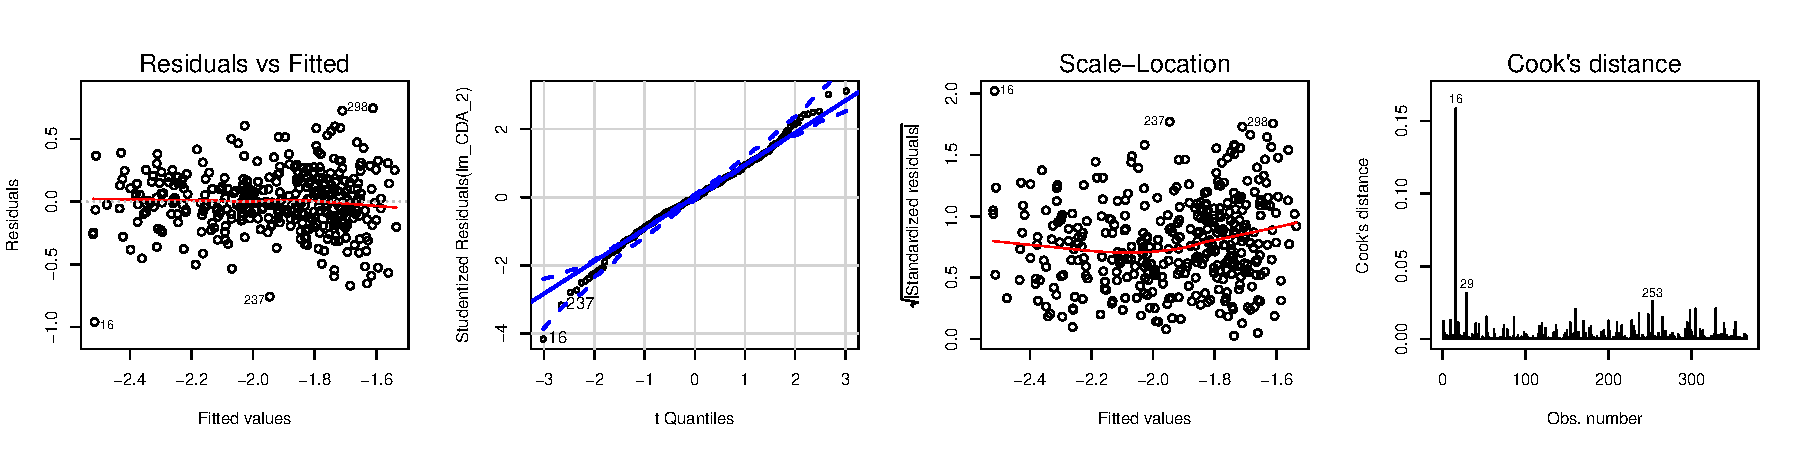
\includegraphics{Report_files/figure-latex/unnamed-chunk-11-1} 

}

\caption{\label{asm}assumptions second model}\label{fig:unnamed-chunk-11}
\end{figure}

The plots in figure \ref{asm} show one big outlier, the municipality
Amsterdam which has number 16. Amsterdams value for the cooks distance
goes way above the cutoff value for cooks, \(4/(369-5-1)=0.011\). It is
also outside the (-3,3) range with the studentized residuals. That is
why this municipality is removed.\\
For the second model without Amsterdam, a step function is used. This
step function uses the AIC for backward elimination. If the AIC can get
lower, because a variable is removed that variable will be removed else
no variable is removed. The formula for AIC is
\(AIC=-2log(likelihood)+2p\), p is the number of parameters in the
model. The variables that are left are the variables used in the final
model.

\begin{verbatim}
## Start:  AIC=-1041.5
## log(CDA_frac) ~ High_educated_frac + Urban_index + Mean_income + 
##     Non_west + Frac_60plus
## 
##                      Df Sum of Sq    RSS     AIC
## - Mean_income         1   0.04208 20.291 -1042.7
## <none>                            20.249 -1041.5
## - High_educated_frac  1   0.36195 20.611 -1037.0
## - Frac_60plus         1   0.67266 20.922 -1031.6
## - Non_west            2   1.54236 21.792 -1018.7
## - Urban_index         1   1.72696 21.976 -1013.6
## 
## Step:  AIC=-1042.74
## log(CDA_frac) ~ High_educated_frac + Urban_index + Non_west + 
##     Frac_60plus
## 
##                      Df Sum of Sq    RSS     AIC
## <none>                            20.291 -1042.7
## - Frac_60plus         1   0.66435 20.956 -1033.0
## - High_educated_frac  1   0.85427 21.146 -1029.7
## - Non_west            2   1.51164 21.803 -1020.5
## - Urban_index         1   1.68687 21.978 -1015.6
\end{verbatim}

\begin{verbatim}
## 
## Call:
## lm(formula = log(CDA_frac) ~ High_educated_frac + Urban_index + 
##     Non_west + Frac_60plus, data = Data_CDA[-16, ])
## 
## Coefficients:
##        (Intercept)  High_educated_frac         Urban_index  
##            -1.0298             -0.8277             -0.1311  
##          Non_west2           Non_west3         Frac_60plus  
##            -0.1141             -0.2871             -3.0168
\end{verbatim}

\subsection{Final model}\label{final-model}

The backward elimination gave the final model.\\
\(ln(Y_i) = \beta_0 + \beta_1*high educated fraction + \beta_2*Urban index + \beta_4*Non west2 + \beta_5*Non west 3 + \beta_6*Frac 60plus + \epsilon i\)
The coëfficients are given in the table below

\begin{table}[ht]
\centering
\begin{tabular}{rrrrr}
  \hline
 & Estimate & Std. Error & t value & Pr($>$$|$t$|$) \\ 
  \hline
(Intercept) & -1.0298 & 0.1365 & -7.54 & 0.0000 \\ 
  High\_educated\_frac & -0.8277 & 0.2129 & -3.89 & 0.0001 \\ 
  Urban\_index & -0.1311 & 0.0240 & -5.46 & 0.0000 \\ 
  Non\_west2 & -0.1141 & 0.0378 & -3.02 & 0.0027 \\ 
  Non\_west3 & -0.2871 & 0.0559 & -5.13 & 0.0000 \\ 
  Frac\_60plus & -3.0168 & 0.8799 & -3.43 & 0.0007 \\ 
   \hline
\end{tabular}
\end{table}

First, the error-assumptions will be checked (figure \ref{afm}). The
`loudspeaker pattern' almost disappeared, so the variance of the error
is almost stable. Because the model is already transformed into a log
model, there is not much transformation possible to let the pattern
totally disappear. The influence will not be that high, because the
pattern is relatively small. In the qq-plot it is visible that almost
all municipalities are in the -3,3 range. Only the municipalities
Oostzaan and Tubbergen are outside this range. This is because Oostzaan
has an extreme low CDA\_frac(0.067) and Tubbergen an extreme high
CDA\_frac(0.42). The decision is made not to delete these values,
because they are still in the 95\% envelope of the qq-plot. In the third
plot the red line is notable, it goes up at the end of the graph. This
means that there is some non-constant error variance, but because the
scatter is not that big no action is needed.

\begin{verbatim}
## 237 298 
## 236 297
\end{verbatim}

\begin{figure}[H]

{\centering 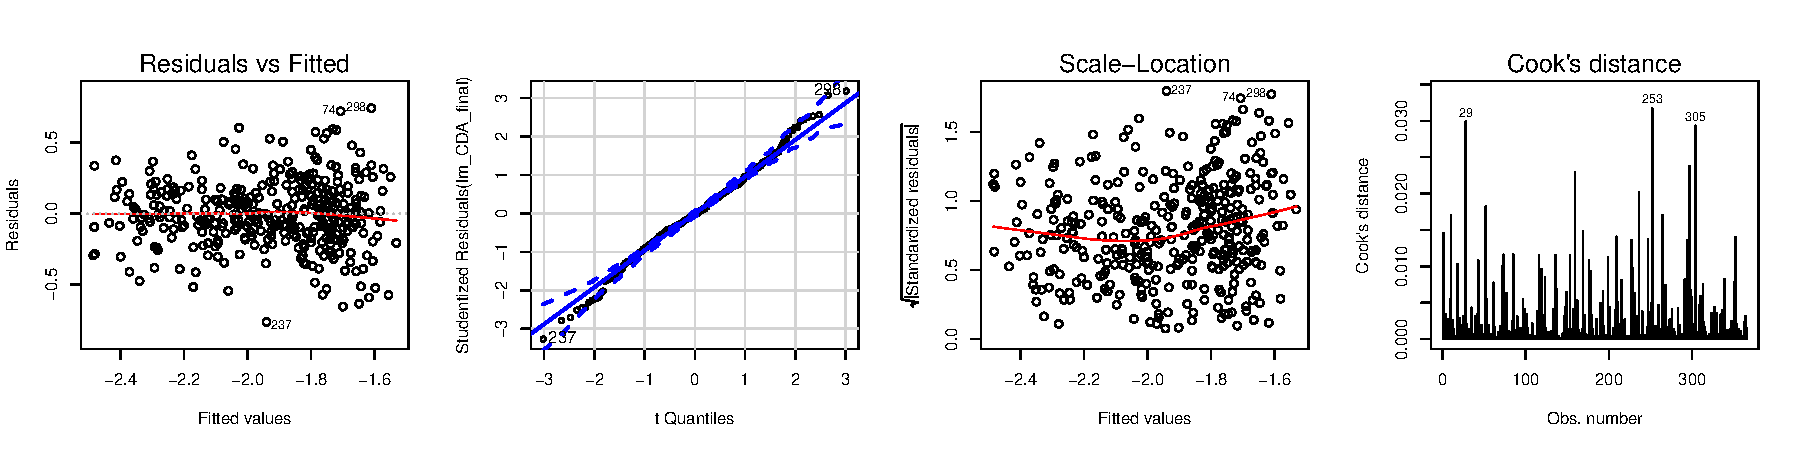
\includegraphics{Report_files/figure-latex/unnamed-chunk-13-1} 

}

\caption{\label{afm}Assumptions final model}\label{fig:unnamed-chunk-13}
\end{figure}

The estimates for the predictors are filled in the model and the
following results are obtained:

\(ln(Y_i) = -1.0298 -0.8277*high educated fraction -0.1311*Urban index -0.1141*Non west2 -0.2871*Non west3 -3.0168*Frac 60plus + \epsilon i\)

Something notable is that all coëfficients are negative, but because the
fitted values are logaritmic the eventual output will be positive. The
added-variable plots are visible below (figure\{avf\}).

\begin{figure}[H]

{\centering 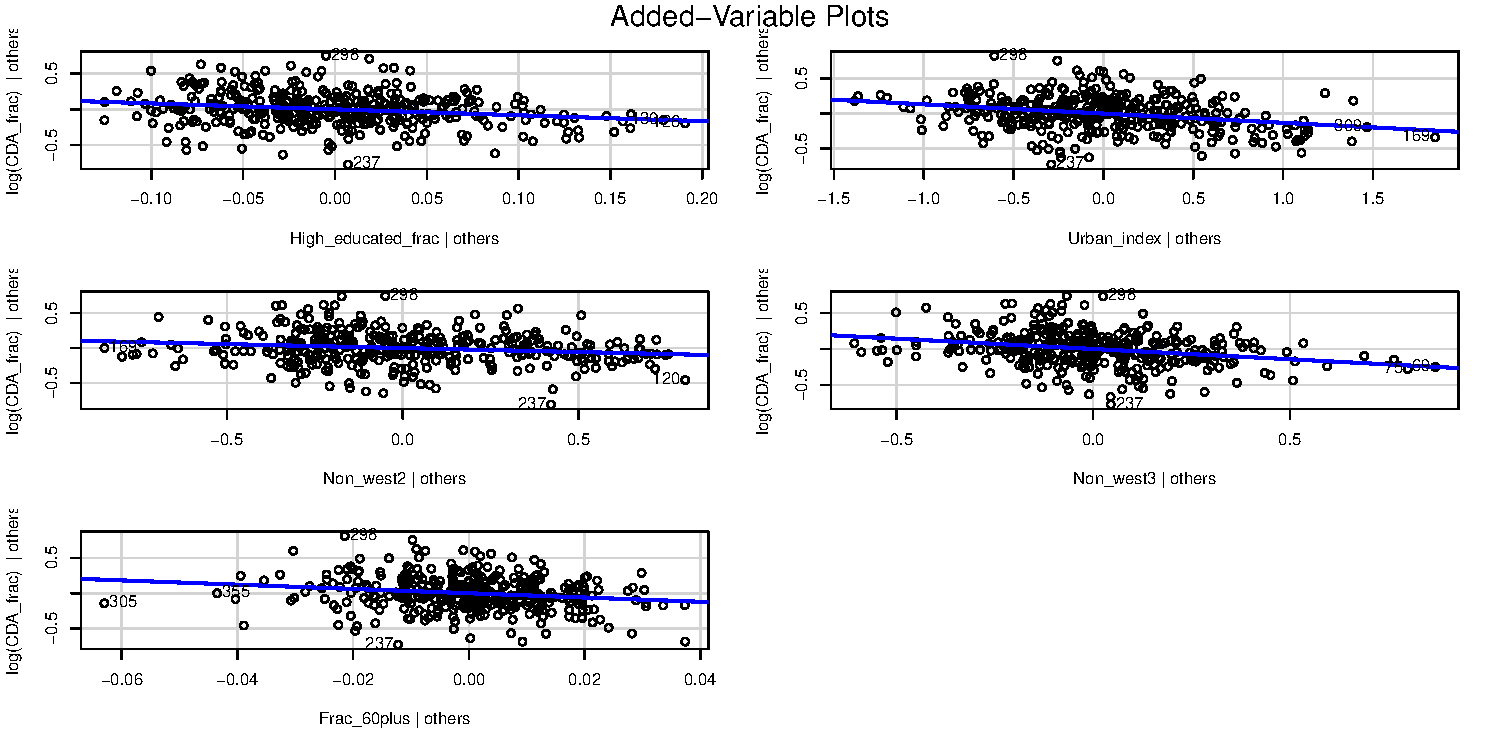
\includegraphics{Report_files/figure-latex/unnamed-chunk-14-1} 

}

\caption{\label{avf} Added variable plots final model}\label{fig:unnamed-chunk-14}
\end{figure}

\subsection{Cross validation}\label{cross-validation}

\section{3. Logistic regression}\label{logistic-regression}

The raw respons variable is the absolute amount of residents per
municipality that voted for CDA. For linear regresssion, this variable
is transformed to a fraction. However, the absolute total amount of
votes per municipality is also available. Therefore, a binomial model
would be a better fit to the data. A second model is developed that uses
the logit as link function to transform the range of the respons. The
choice for the logit was easily made. Because the inverse of the logit
is directly interpretable as the log-odds ratio. This link displays the
underlaying pattern of this data best. Below, the formula for the link
function:

\(\eta = log(\frac{\theta}{1 - \theta}) = \beta_0 + \beta_1 x_1 + \beta_2 x_2 + ... + \beta_n x_n\)

Where \(\theta\) is the probability of votes for CDA.

Also for logistics regression are diagnostic plots needed to visualise
the deviance/pearson residuals and search for outliers. Most of the
diagnostics from the linear model extend relatively straighforward to
logistic regression. However, leverages are no longer just a function of
the explanatory variable, but also depend on the respons due to iterated
weighted least squares. Furthermore, \(\theta\) can never be zero or
one. Fortunately, this was not the case for any of the observations in
this dataset.

\subsection{First model}\label{first-model-1}

Again, the first is the full model. Stepwise backward elimination is
used to find the optimal model. Below, the formula for the full model:

\(log(\frac{\theta}{1 - \theta}) = \beta_0 + \beta_1 \cdot UrbanIndex + \beta_2 \cdot HighlyEducatedFraction + \beta_3 \cdot MeanIncome + \beta_4 \cdot NonWest + \beta_5 \cdot Fraction60Plus\)

\begin{Shaded}
\begin{Highlighting}[]
\NormalTok{glm_CDA_}\DecValTok{1}\NormalTok{ <-}\StringTok{ }\KeywordTok{glm}\NormalTok{(}\KeywordTok{cbind}\NormalTok{(CDA_abs, Total_abs }\OperatorTok{-}\StringTok{ }\NormalTok{CDA_abs) }\OperatorTok{~}\StringTok{ }\NormalTok{Urban_index }\OperatorTok{+}\StringTok{ }\NormalTok{High_educated_frac }\OperatorTok{+}\StringTok{ }
\StringTok{    }\NormalTok{Mean_income }\OperatorTok{+}\StringTok{ }\NormalTok{Non_west }\OperatorTok{+}\StringTok{ }\NormalTok{Frac_60plus, }\DataTypeTok{family =} \KeywordTok{binomial}\NormalTok{(}\DataTypeTok{link =} \StringTok{"logit"}\NormalTok{), }
    \DataTypeTok{data =}\NormalTok{ Data_CDA)}
\KeywordTok{summary}\NormalTok{(glm_CDA_}\DecValTok{1}\NormalTok{)}
\end{Highlighting}
\end{Shaded}

\begin{verbatim}
## 
## Call:
## glm(formula = cbind(CDA_abs, Total_abs - CDA_abs) ~ Urban_index + 
##     High_educated_frac + Mean_income + Non_west + Frac_60plus, 
##     family = binomial(link = "logit"), data = Data_CDA)
## 
## Deviance Residuals: 
##     Min       1Q   Median       3Q      Max  
## -88.318   -8.988   -1.521    7.670   57.920  
## 
## Coefficients:
##                      Estimate Std. Error z value Pr(>|z|)    
## (Intercept)        -1.0559765  0.0156927  -67.29   <2e-16 ***
## Urban_index        -0.1933926  0.0020376  -94.91   <2e-16 ***
## High_educated_frac -2.1027583  0.0199536 -105.38   <2e-16 ***
## Mean_income         0.0156359  0.0005334   29.32   <2e-16 ***
## Non_west2          -0.0562758  0.0031606  -17.80   <2e-16 ***
## Non_west3          -0.2592768  0.0046088  -56.26   <2e-16 ***
## Frac_60plus        -1.3424322  0.0737404  -18.20   <2e-16 ***
## ---
## Signif. codes:  0 '***' 0.001 '**' 0.01 '*' 0.05 '.' 0.1 ' ' 1
## 
## (Dispersion parameter for binomial family taken to be 1)
## 
##     Null deviance: 247550  on 365  degrees of freedom
## Residual deviance:  89969  on 359  degrees of freedom
## AIC: 93475
## 
## Number of Fisher Scoring iterations: 4
\end{verbatim}

The summary visualizes that the all the variables are very significant,
with small errors. The full model has 359 degrees of freedom and it is
expected that the residual deviance is roughly equivalent. However, the
residual deviance is far above this value. These are strong indications
that this model suffers from overdispersion. This assumption seems
reasonable, because there is a very large variance in how many residents
per municapality voted for CDA. In some municipalities only 3\% voted
for CDA, while it others nearly 50\% voted for CDA. It is concluded that
a quasi-binomial would fit the data better.

\subsection{Second model}\label{second-model-1}

\begin{Shaded}
\begin{Highlighting}[]
\NormalTok{glm_CDA_}\DecValTok{2}\NormalTok{ <-}\StringTok{ }\KeywordTok{glm}\NormalTok{(}\KeywordTok{cbind}\NormalTok{(CDA_abs, Total_abs }\OperatorTok{-}\StringTok{ }\NormalTok{CDA_abs) }\OperatorTok{~}\StringTok{ }\NormalTok{Urban_index }\OperatorTok{+}\StringTok{ }\NormalTok{High_educated_frac }\OperatorTok{+}\StringTok{ }
\StringTok{    }\NormalTok{Mean_income }\OperatorTok{+}\StringTok{ }\NormalTok{Non_west }\OperatorTok{+}\StringTok{ }\NormalTok{Frac_60plus, }\DataTypeTok{family =} \KeywordTok{quasibinomial}\NormalTok{(}\DataTypeTok{link =} \StringTok{"logit"}\NormalTok{), }
    \DataTypeTok{data =}\NormalTok{ Data_CDA)}
\KeywordTok{summary}\NormalTok{(glm_CDA_}\DecValTok{2}\NormalTok{)}
\end{Highlighting}
\end{Shaded}

\begin{verbatim}
## 
## Call:
## glm(formula = cbind(CDA_abs, Total_abs - CDA_abs) ~ Urban_index + 
##     High_educated_frac + Mean_income + Non_west + Frac_60plus, 
##     family = quasibinomial(link = "logit"), data = Data_CDA)
## 
## Deviance Residuals: 
##     Min       1Q   Median       3Q      Max  
## -88.318   -8.988   -1.521    7.670   57.920  
## 
## Coefficients:
##                     Estimate Std. Error t value Pr(>|t|)    
## (Intercept)        -1.055977   0.250122  -4.222 3.07e-05 ***
## Urban_index        -0.193393   0.032478  -5.955 6.21e-09 ***
## High_educated_frac -2.102758   0.318036  -6.612 1.38e-10 ***
## Mean_income         0.015636   0.008501   1.839  0.06670 .  
## Non_west2          -0.056276   0.050376  -1.117  0.26469    
## Non_west3          -0.259277   0.073459  -3.530  0.00047 ***
## Frac_60plus        -1.342432   1.175330  -1.142  0.25414    
## ---
## Signif. codes:  0 '***' 0.001 '**' 0.01 '*' 0.05 '.' 0.1 ' ' 1
## 
## (Dispersion parameter for quasibinomial family taken to be 254.0441)
## 
##     Null deviance: 247550  on 365  degrees of freedom
## Residual deviance:  89969  on 359  degrees of freedom
## AIC: NA
## 
## Number of Fisher Scoring iterations: 4
\end{verbatim}

By applying a quasi binomial model, a dispersion parameter \(\phi\) is
included, resulting in larger standard errors and less significant
p-values. \(\phi\) is estimated on the data at 254.0441. The variables
\texttt{Frac\_60plus}, \texttt{Mean\_income} and factor
\texttt{Non\_west2} are no longer significant.

No goodness of fit test is possible because of the free dispersion
parameter.The decision to remove variables is done based on the lowest
F-test.

\begin{Shaded}
\begin{Highlighting}[]
\KeywordTok{vif}\NormalTok{(glm_CDA_}\DecValTok{2}\NormalTok{)}
\end{Highlighting}
\end{Shaded}

\begin{verbatim}
##        Urban_index High_educated_frac        Mean_income 
##       0.0013605627       0.0005943712       0.0006876039 
##          Non_west2          Non_west3        Frac_60plus 
##       0.0007725368       0.0012914703       0.0005161910
\end{verbatim}

\begin{Shaded}
\begin{Highlighting}[]
\KeywordTok{drop1}\NormalTok{(glm_CDA_}\DecValTok{2}\NormalTok{, }\DataTypeTok{test =} \StringTok{"F"}\NormalTok{)}
\end{Highlighting}
\end{Shaded}

\begin{verbatim}
## Single term deletions
## 
## Model:
## cbind(CDA_abs, Total_abs - CDA_abs) ~ Urban_index + High_educated_frac + 
##     Mean_income + Non_west + Frac_60plus
##                    Df Deviance F value    Pr(>F)    
## <none>                   89969                      
## Urban_index         1    99052 36.2459 4.300e-09 ***
## High_educated_frac  1   101151 44.6196 9.132e-11 ***
## Mean_income         1    90821  3.3987 0.0660730 .  
## Non_west            2    94112  8.2661 0.0003092 ***
## Frac_60plus         1    90300  1.3217 0.2510613    
## ---
## Signif. codes:  0 '***' 0.001 '**' 0.01 '*' 0.05 '.' 0.1 ' ' 1
\end{verbatim}

According to the F-test \texttt{Frac\_60plus} should be removed. This
variable has a F-value of 1.32 and a corresponding p-value of 0.25. The
values for the VIF are all very low, meaning there is barely
collinearity between the explanatory variables.

At last, the residuals and cook's distance are visualized

\begin{Shaded}
\begin{Highlighting}[]
\KeywordTok{par}\NormalTok{(}\DataTypeTok{mfrow =} \KeywordTok{c}\NormalTok{(}\DecValTok{1}\NormalTok{, }\DecValTok{3}\NormalTok{))}
\KeywordTok{halfnorm}\NormalTok{(}\KeywordTok{residuals}\NormalTok{(glm_CDA_}\DecValTok{2}\NormalTok{, }\StringTok{"pearson"}\NormalTok{))}
\KeywordTok{plot}\NormalTok{(glm_CDA_}\DecValTok{2}\NormalTok{, }\DataTypeTok{which =} \DecValTok{1}\NormalTok{, }\DataTypeTok{id.n =} \DecValTok{5}\NormalTok{)}
\KeywordTok{plot}\NormalTok{(glm_CDA_}\DecValTok{2}\NormalTok{, }\DataTypeTok{which =} \DecValTok{4}\NormalTok{, }\DataTypeTok{id.n =} \DecValTok{5}\NormalTok{)}
\end{Highlighting}
\end{Shaded}

\begin{center}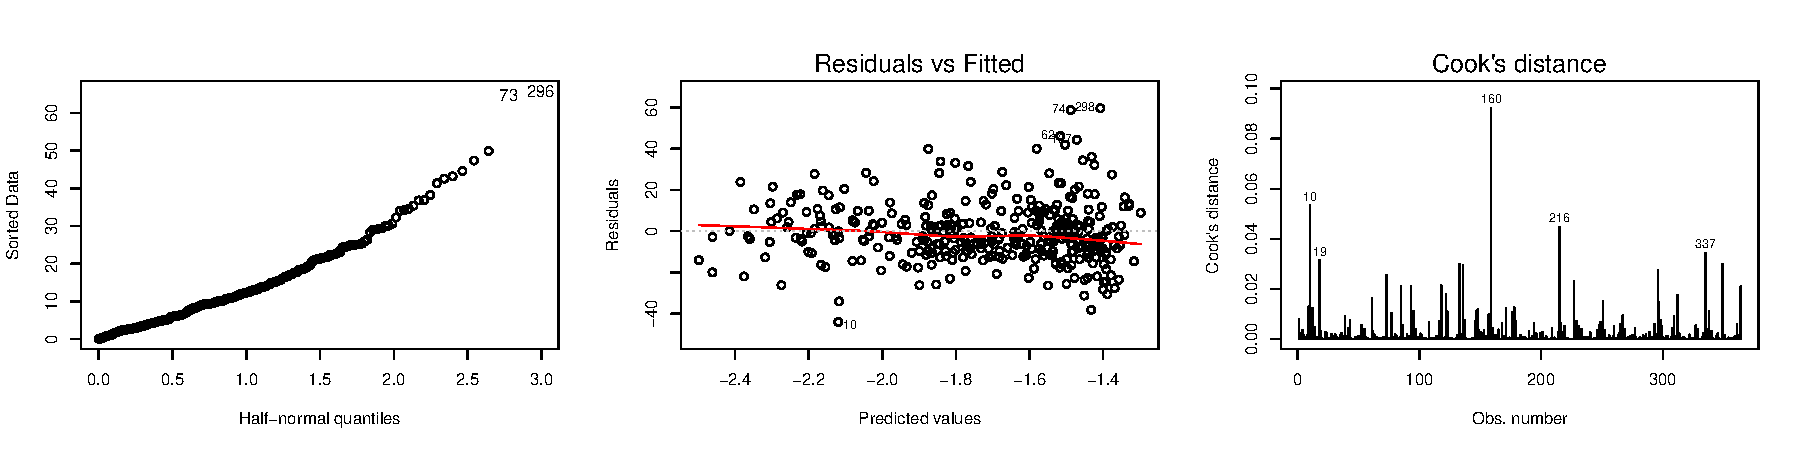
\includegraphics{Report_files/figure-latex/unnamed-chunk-19-1} \end{center}

\begin{Shaded}
\begin{Highlighting}[]
\NormalTok{Data_CDA[}\KeywordTok{c}\NormalTok{(}\DecValTok{16}\NormalTok{, }\DecValTok{74}\NormalTok{, }\DecValTok{265}\NormalTok{), ]}
\end{Highlighting}
\end{Shaded}

\begin{verbatim}
##           Muni CDA_frac Urban_index High_educated_frac Mean_income
## 16   Amsterdam    0.031       3.789               0.47        25.3
## 74  Dinkelland    0.373       0.531               0.26        26.0
## 265  Rotterdam    0.060       3.546               0.31        22.9
##     Non_west_frac CDA_abs Total_abs Frac_60plus Non_west
## 16           0.35   13562    440854        0.09        3
## 74           0.02    6560     17586        0.13        1
## 265          0.38   18813    315550        0.10        3
\end{verbatim}

The left plot display the half-normal quantiles against the pearson
residuals. Ideally, these residuals would not be greater than 3.
However, this plot shows residuals even up to 80. The middle plot
displays the predicted values against the deviance resiuals. Also here a
large spread of the residuals is observed. There seems to be
non-constant erro variance, because the spread becomes larger for higher
predicted values. The right plots shows the cook's distance, which can
identify influential observations. Observation 16 is an outlier, because
it is very influential and stands out from any pattern in the residual
plots. Furthermore, Dinkelland (obs 74) and Rotterdam (obs 265) are also
influential. Amsterdam is the municipality with the lowest percentage of
CDA votes and Dinkelland has the highest percentage of CDA votes.

\begin{Shaded}
\begin{Highlighting}[]
\KeywordTok{avPlots}\NormalTok{(glm_CDA_}\DecValTok{2}\NormalTok{)}
\end{Highlighting}
\end{Shaded}

\begin{center}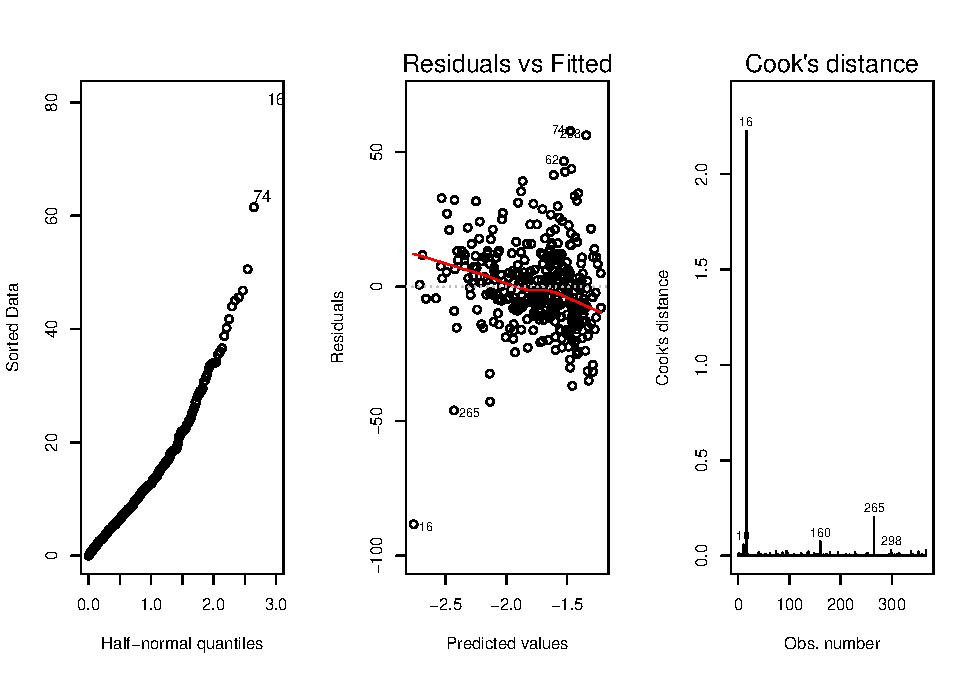
\includegraphics{Report_files/figure-latex/unnamed-chunk-20-1} \end{center}

The avPlots help to interpret the partial regression coefficients when
the other variables are held constant.The partial regression line is
highly influenced by observation 16 again. The blue lines do not
represent the data well at the moment.

\subsection{Third model}\label{third-model}

For this model the variable \texttt{Frac\_60plus} is removed, because it
had the lowest F-value. Furthermore, the observations 16 (Amsterdam) and
265 (Dinkelland) are removed. These influenced the partial regression
coefficients greatly and had large residual and cook's distances. These
steps were originally done in two, but they are combined for this
report.

\begin{Shaded}
\begin{Highlighting}[]
\NormalTok{glm_CDA_}\DecValTok{4}\NormalTok{ <-}\StringTok{ }\KeywordTok{glm}\NormalTok{(}\KeywordTok{cbind}\NormalTok{(CDA_abs, Total_abs }\OperatorTok{-}\StringTok{ }\NormalTok{CDA_abs) }\OperatorTok{~}\StringTok{ }\NormalTok{Urban_index }\OperatorTok{+}\StringTok{ }\NormalTok{High_educated_frac }\OperatorTok{+}\StringTok{ }
\StringTok{    }\NormalTok{Mean_income }\OperatorTok{+}\StringTok{ }\NormalTok{Non_west, }\DataTypeTok{family =} \KeywordTok{quasibinomial}\NormalTok{(}\DataTypeTok{link =} \StringTok{"logit"}\NormalTok{), }\DataTypeTok{data =}\NormalTok{ Data_CDA[}\OperatorTok{-}\KeywordTok{c}\NormalTok{(}\DecValTok{16}\NormalTok{, }
    \DecValTok{265}\NormalTok{), ])}
\KeywordTok{summary}\NormalTok{(glm_CDA_}\DecValTok{4}\NormalTok{)}
\end{Highlighting}
\end{Shaded}

\begin{verbatim}
## 
## Call:
## glm(formula = cbind(CDA_abs, Total_abs - CDA_abs) ~ Urban_index + 
##     High_educated_frac + Mean_income + Non_west, family = quasibinomial(link = "logit"), 
##     data = Data_CDA[-c(16, 265), ])
## 
## Deviance Residuals: 
##     Min       1Q   Median       3Q      Max  
## -44.024   -9.619   -2.437    6.074   59.653  
## 
## Coefficients:
##                      Estimate Std. Error t value Pr(>|t|)    
## (Intercept)        -1.0877540  0.1801672  -6.037 3.92e-09 ***
## Urban_index        -0.1351943  0.0303257  -4.458 1.11e-05 ***
## High_educated_frac -1.2202265  0.3125548  -3.904 0.000113 ***
## Mean_income        -0.0004273  0.0081731  -0.052 0.958331    
## Non_west2          -0.1232492  0.0479004  -2.573 0.010483 *  
## Non_west3          -0.3447138  0.0690753  -4.990 9.42e-07 ***
## ---
## Signif. codes:  0 '***' 0.001 '**' 0.01 '*' 0.05 '.' 0.1 ' ' 1
## 
## (Dispersion parameter for quasibinomial family taken to be 221.709)
## 
##     Null deviance: 173842  on 363  degrees of freedom
## Residual deviance:  76966  on 358  degrees of freedom
## AIC: NA
## 
## Number of Fisher Scoring iterations: 4
\end{verbatim}

By removing observation 16 and 265, the factor \texttt{Non\_west2} has
become significant. Also the residual deviance has decreased slightly,
but is still far above the degrees of freedom.

\begin{Shaded}
\begin{Highlighting}[]
\KeywordTok{par}\NormalTok{(}\DataTypeTok{mfrow =} \KeywordTok{c}\NormalTok{(}\DecValTok{1}\NormalTok{, }\DecValTok{3}\NormalTok{))}
\KeywordTok{halfnorm}\NormalTok{(}\KeywordTok{residuals}\NormalTok{(glm_CDA_}\DecValTok{4}\NormalTok{, }\StringTok{"pearson"}\NormalTok{))}
\KeywordTok{plot}\NormalTok{(glm_CDA_}\DecValTok{4}\NormalTok{, }\DataTypeTok{which =} \DecValTok{1}\NormalTok{, }\DataTypeTok{id.n =} \DecValTok{5}\NormalTok{)}
\KeywordTok{plot}\NormalTok{(glm_CDA_}\DecValTok{4}\NormalTok{, }\DataTypeTok{which =} \DecValTok{4}\NormalTok{, }\DataTypeTok{id.n =} \DecValTok{5}\NormalTok{)}
\end{Highlighting}
\end{Shaded}

\begin{center}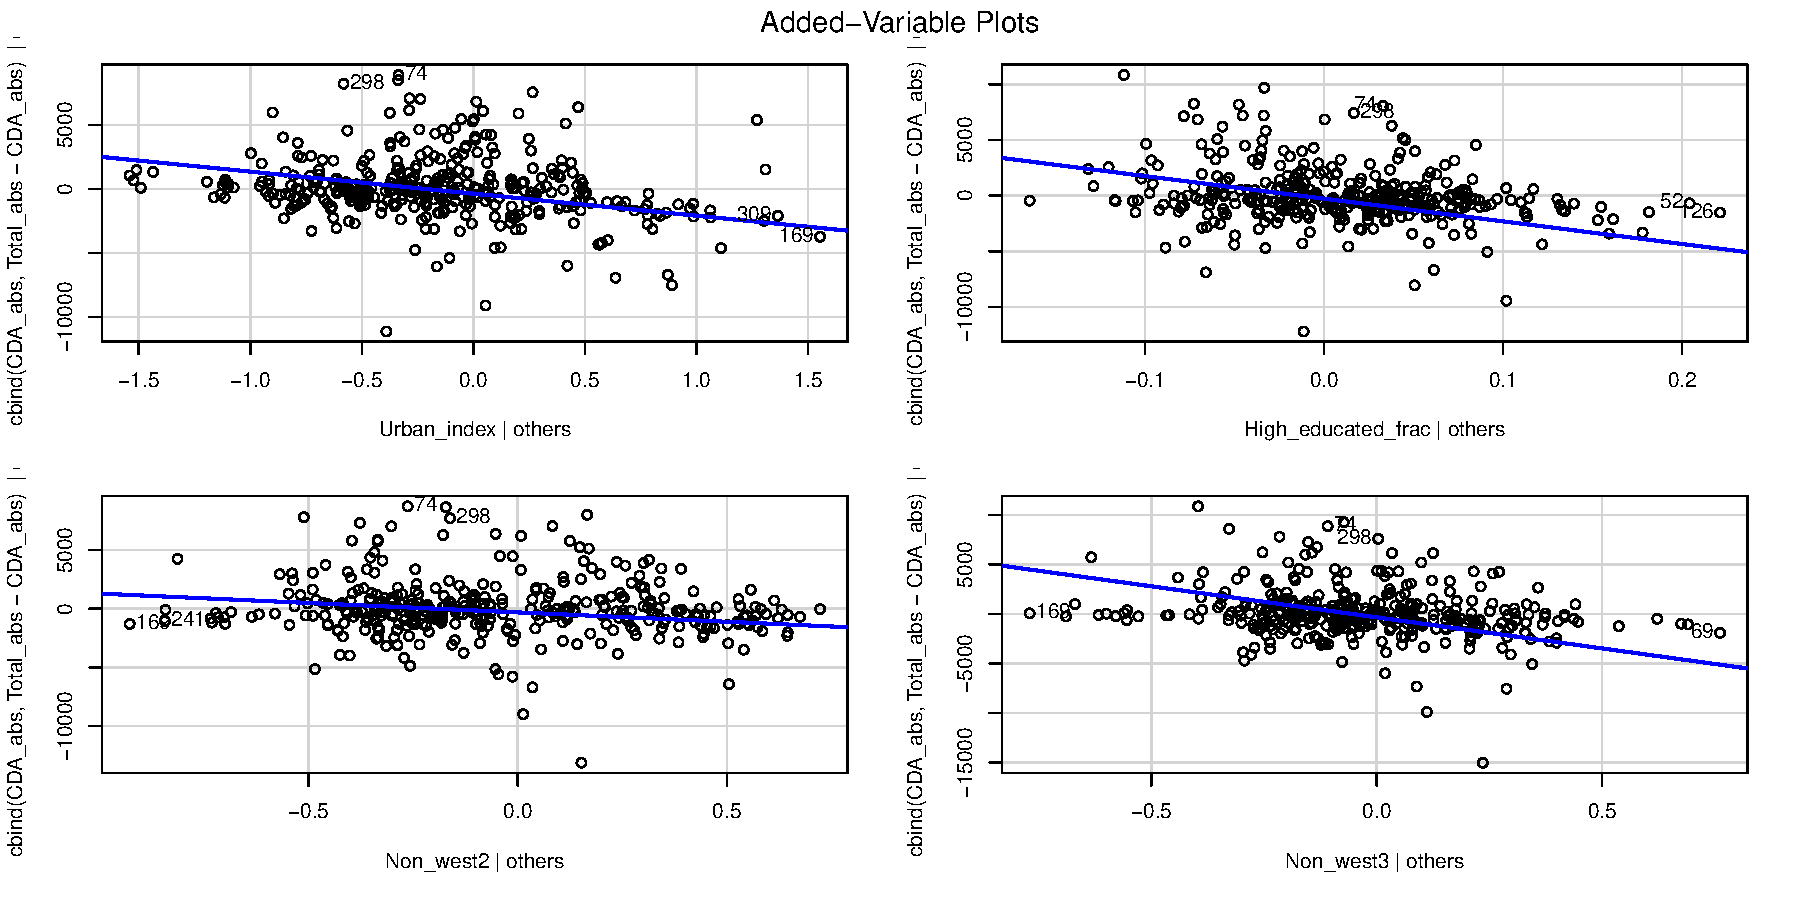
\includegraphics{Report_files/figure-latex/unnamed-chunk-22-1} \end{center}

The plot left still displays very large pearson residuals. The plot in
the middle seems homogenic distributed, which slightly more variance for
higher predicted values. And the cook's distance no longer displays
highly influential observations.

\begin{Shaded}
\begin{Highlighting}[]
\KeywordTok{drop1}\NormalTok{(glm_CDA_}\DecValTok{4}\NormalTok{, }\DataTypeTok{test =} \StringTok{"F"}\NormalTok{)}
\end{Highlighting}
\end{Shaded}

\begin{verbatim}
## Single term deletions
## 
## Model:
## cbind(CDA_abs, Total_abs - CDA_abs) ~ Urban_index + High_educated_frac + 
##     Mean_income + Non_west
##                    Df Deviance F value    Pr(>F)    
## <none>                   76966                      
## Urban_index         1    81396 20.6048 7.721e-06 ***
## High_educated_frac  1    80361 15.7942 8.543e-05 ***
## Mean_income         1    76966  0.0028    0.9577    
## Non_west            2    82994 14.0208 1.373e-06 ***
## ---
## Signif. codes:  0 '***' 0.001 '**' 0.01 '*' 0.05 '.' 0.1 ' ' 1
\end{verbatim}

According to the F-test \texttt{Mean\_income} should be removed as well,
because the F-value is below 1 and the corresponding p-value is 0.96.

\subsection{Final model}\label{final-model-1}

The final model is reached after dropping the variables
\texttt{Mean\_income} and \texttt{Frac\_60plus}. It's formula is as
follows:

\(logit(p_{ij}) = -1.09 -0.14 \cdot UrbanIndex -1.23 \cdot HighlyEducatedFraction - 0.12 \cdot NonWest:2 - 0.34 \cdot NonWest:3\)

\begin{Shaded}
\begin{Highlighting}[]
\NormalTok{glm_CDA_}\DecValTok{5}\NormalTok{ <-}\StringTok{ }\KeywordTok{glm}\NormalTok{(}\KeywordTok{cbind}\NormalTok{(CDA_abs, Total_abs }\OperatorTok{-}\StringTok{ }\NormalTok{CDA_abs) }\OperatorTok{~}\StringTok{ }\NormalTok{Urban_index }\OperatorTok{+}\StringTok{ }\NormalTok{High_educated_frac }\OperatorTok{+}\StringTok{ }
\StringTok{    }\NormalTok{Non_west, }\DataTypeTok{family =} \KeywordTok{quasibinomial}\NormalTok{(}\DataTypeTok{link =} \StringTok{"logit"}\NormalTok{), }\DataTypeTok{data =}\NormalTok{ Data_CDA[}\OperatorTok{-}\KeywordTok{c}\NormalTok{(}\DecValTok{16}\NormalTok{, }
    \DecValTok{265}\NormalTok{), ])}
\KeywordTok{summary}\NormalTok{(glm_CDA_}\DecValTok{5}\NormalTok{)}
\end{Highlighting}
\end{Shaded}

\begin{verbatim}
## 
## Call:
## glm(formula = cbind(CDA_abs, Total_abs - CDA_abs) ~ Urban_index + 
##     High_educated_frac + Non_west, family = quasibinomial(link = "logit"), 
##     data = Data_CDA[-c(16, 265), ])
## 
## Deviance Residuals: 
##     Min       1Q   Median       3Q      Max  
## -44.014   -9.626   -2.447    6.099   59.654  
## 
## Coefficients:
##                    Estimate Std. Error t value Pr(>|t|)    
## (Intercept)        -1.09653    0.06526 -16.804  < 2e-16 ***
## Urban_index        -0.13497    0.02996  -4.504 9.02e-06 ***
## High_educated_frac -1.22972    0.25406  -4.840 1.93e-06 ***
## Non_west2          -0.12346    0.04767  -2.590  0.00999 ** 
## Non_west3          -0.34443    0.06876  -5.009 8.60e-07 ***
## ---
## Signif. codes:  0 '***' 0.001 '**' 0.01 '*' 0.05 '.' 0.1 ' ' 1
## 
## (Dispersion parameter for quasibinomial family taken to be 221.0972)
## 
##     Null deviance: 173842  on 363  degrees of freedom
## Residual deviance:  76966  on 359  degrees of freedom
## AIC: NA
## 
## Number of Fisher Scoring iterations: 4
\end{verbatim}

\begin{Shaded}
\begin{Highlighting}[]
\KeywordTok{drop1}\NormalTok{(glm_CDA_}\DecValTok{5}\NormalTok{, }\DataTypeTok{test =} \StringTok{"F"}\NormalTok{)}
\end{Highlighting}
\end{Shaded}

\begin{verbatim}
## Single term deletions
## 
## Model:
## cbind(CDA_abs, Total_abs - CDA_abs) ~ Urban_index + High_educated_frac + 
##     Non_west
##                    Df Deviance F value    Pr(>F)    
## <none>                   76966                      
## Urban_index         1    81471  21.009 6.318e-06 ***
## High_educated_frac  1    82190  24.364 1.223e-06 ***
## Non_west            2    83077  14.251 1.108e-06 ***
## ---
## Signif. codes:  0 '***' 0.001 '**' 0.01 '*' 0.05 '.' 0.1 ' ' 1
\end{verbatim}

The F-test shows that all variables now significantly contribute to the
model. The residual deviance has slightly decreased, in compare to model
\texttt{glm\_CDA\_2} with all the variables. However, the residual
deviance is still much larger then the degrees of freedom.

\begin{Shaded}
\begin{Highlighting}[]
\KeywordTok{par}\NormalTok{(}\DataTypeTok{mfrow =} \KeywordTok{c}\NormalTok{(}\DecValTok{1}\NormalTok{, }\DecValTok{3}\NormalTok{))}
\KeywordTok{halfnorm}\NormalTok{(}\KeywordTok{residuals}\NormalTok{(glm_CDA_}\DecValTok{5}\NormalTok{, }\StringTok{"pearson"}\NormalTok{))}
\KeywordTok{plot}\NormalTok{(glm_CDA_}\DecValTok{5}\NormalTok{, }\DataTypeTok{which =} \DecValTok{1}\NormalTok{, }\DataTypeTok{id.n =} \DecValTok{5}\NormalTok{)}
\KeywordTok{plot}\NormalTok{(glm_CDA_}\DecValTok{5}\NormalTok{, }\DataTypeTok{which =} \DecValTok{4}\NormalTok{, }\DataTypeTok{id.n =} \DecValTok{5}\NormalTok{)}
\end{Highlighting}
\end{Shaded}

\begin{center}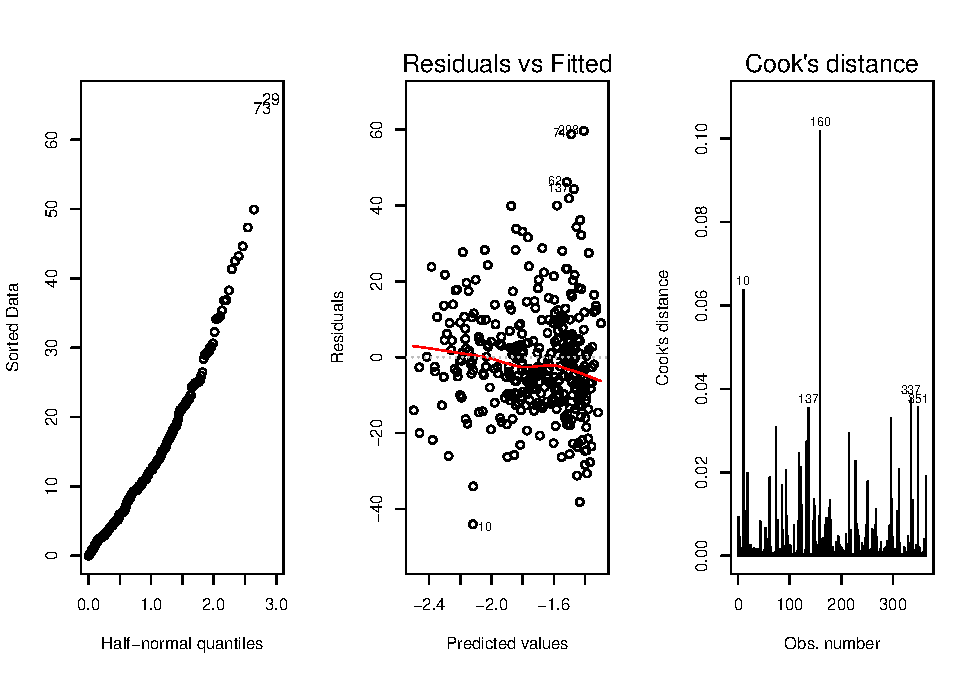
\includegraphics{Report_files/figure-latex/unnamed-chunk-25-1} \end{center}

There is still a large spread of both the pearson (left plot) and
deviance (middle plot) residuals. Furthermore, there is non-constant
errror variance. The cook's distance does not display very influential
observations.

\begin{Shaded}
\begin{Highlighting}[]
\KeywordTok{vif}\NormalTok{(glm_CDA_}\DecValTok{5}\NormalTok{)}
\end{Highlighting}
\end{Shaded}

\begin{verbatim}
##        Urban_index High_educated_frac          Non_west2 
##       0.0012896670       0.0004230904       0.0007928046 
##          Non_west3 
##       0.0012734699
\end{verbatim}

\begin{Shaded}
\begin{Highlighting}[]
\KeywordTok{avPlots}\NormalTok{(glm_CDA_}\DecValTok{5}\NormalTok{)}
\end{Highlighting}
\end{Shaded}

\begin{center}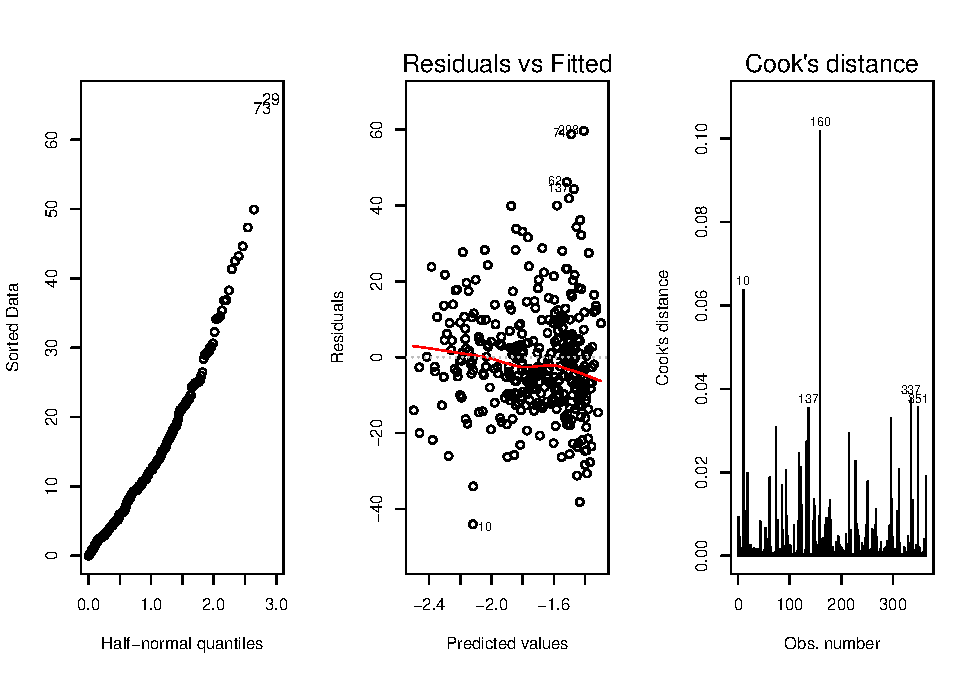
\includegraphics{Report_files/figure-latex/unnamed-chunk-26-1} \end{center}

After removing two outliers, the partial regression coefficients
represent the data much better. There are no strong correlations between
the explanatory variables and the respons. The low VIF values also
indicate this.

\begin{Shaded}
\begin{Highlighting}[]
\NormalTok{function_nonwest1 <-}\StringTok{ }\ControlFlowTok{function}\NormalTok{(x) \{}
    \OperatorTok{-}\FloatTok{1.09} \OperatorTok{-}\StringTok{ }\FloatTok{0.14} \OperatorTok{*}\StringTok{ }\NormalTok{x }\OperatorTok{-}\StringTok{ }\FloatTok{1.23} \OperatorTok{*}\StringTok{ }\NormalTok{x}
\NormalTok{\}}
\NormalTok{function_nonwest2 <-}\StringTok{ }\ControlFlowTok{function}\NormalTok{(x) \{}
    \OperatorTok{-}\FloatTok{1.09} \OperatorTok{-}\StringTok{ }\FloatTok{0.14} \OperatorTok{*}\StringTok{ }\NormalTok{x }\OperatorTok{-}\StringTok{ }\FloatTok{1.23} \OperatorTok{*}\StringTok{ }\NormalTok{x }\OperatorTok{-}\StringTok{ }\FloatTok{0.12} \OperatorTok{*}\StringTok{ }\NormalTok{x}
\NormalTok{\}}
\NormalTok{function_nonwest3 <-}\StringTok{ }\ControlFlowTok{function}\NormalTok{(x) \{}
    \OperatorTok{-}\FloatTok{1.09} \OperatorTok{-}\StringTok{ }\FloatTok{0.14} \OperatorTok{*}\StringTok{ }\NormalTok{x }\OperatorTok{-}\StringTok{ }\FloatTok{1.23} \OperatorTok{*}\StringTok{ }\NormalTok{x }\OperatorTok{-}\StringTok{ }\FloatTok{0.34} \OperatorTok{*}\StringTok{ }\NormalTok{x}
\NormalTok{\}}
\KeywordTok{plot}\NormalTok{(}\KeywordTok{function_nonwest1}\NormalTok{(}\DecValTok{1}\OperatorTok{:}\DecValTok{10}\NormalTok{), }\DataTypeTok{type =} \StringTok{"l"}\NormalTok{)}
\KeywordTok{lines}\NormalTok{(}\KeywordTok{function_nonwest2}\NormalTok{(}\DecValTok{1}\OperatorTok{:}\DecValTok{10}\NormalTok{), }\DataTypeTok{type =} \StringTok{"l"}\NormalTok{, }\DataTypeTok{col =} \StringTok{"red"}\NormalTok{)}
\KeywordTok{lines}\NormalTok{(}\KeywordTok{function_nonwest3}\NormalTok{(}\DecValTok{1}\OperatorTok{:}\DecValTok{10}\NormalTok{), }\DataTypeTok{type =} \StringTok{"l"}\NormalTok{, }\DataTypeTok{col =} \StringTok{"blue"}\NormalTok{)}
\end{Highlighting}
\end{Shaded}

\begin{center}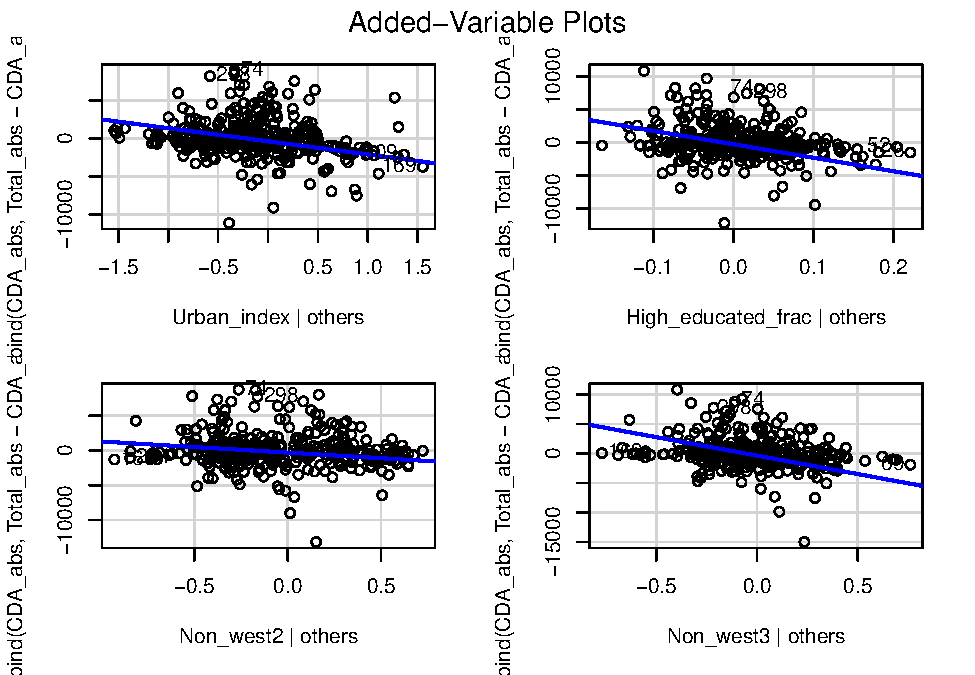
\includegraphics{Report_files/figure-latex/unnamed-chunk-27-1} \end{center}

\subsection{Cross validation}\label{cross-validation-1}

\section{4. Discussion}\label{discussion}

\subsection{Limitations}\label{limitations}


\end{document}
